%% Based on a TeXnicCenter-Template by Tino Weinkauf.
%%%%%%%%%%%%%%%%%%%%%%%%%%%%%%%%%%%%%%%%%%%%%%%%%%%%%%%%%%%%%

%%%%%%%%%%%%%%%%%%%%%%%%%%%%%%%%%%%%%%%%%%%%%%%%%%%%%%%%%%%%%
%% HEADER
%%%%%%%%%%%%%%%%%%%%%%%%%%%%%%%%%%%%%%%%%%%%%%%%%%%%%%%%%%%%%
\documentclass[a4paper,twoside,10pt]{report}
% Alternative Options:
%	Paper Size: a4paper / a5paper / b5paper / letterpaper / legalpaper / executivepaper
% Duplex: oneside / twoside
% Base Font Size: 10pt / 11pt / 12pt


%% Language %%%%%%%%%%%%%%%%%%%%%%%%%%%%%%%%%%%%%%%%%%%%%%%%%
\usepackage[english]{babel}	% put only one language here
\selectlanguage{english}			% f�r silbentrennung und neue deutsche rechtschreibung

\usepackage[dvips]{graphicx}
\usepackage{array}		% extrarowheight of tables
\usepackage{graphicx}   % eps import	
\usepackage[savemem,final]{listings}	% code listings
\usepackage{fancyhdr}	% for nicer headers
\usepackage{caption}
\usepackage{color}
\usepackage{url}
\usepackage{marvosym}	% for the stop symbol warning about important things
\usepackage{mparhack}				% notifies about changes in marginpar - layout
\usepackage{xspace}	% variable space after e.g. abbreviations
\usepackage{here}
\usepackage{lettrine}
\usepackage[]{algorithm2e}

% global settings
\pagestyle{headings}  
\graphicspath{{gfx/}}
%\DeclareGraphicsExtensions{.eps,.pdf,.png}
%\DeclareGraphicsRule{.eps}{eps}{.eps}{}
%\DeclareGraphicsRule{.pdf}{pdf}{.pdf}{}
%\DeclareGraphicsRule{.png}{png}{.png}{}


\usepackage{lmodern} %Type1-font for non-english texts and characters


%% Packages for Graphics & Figures %%%%%%%%%%%%%%%%%%%%%%%%%%
\usepackage{graphicx} %%For loading graphic files
%\usepackage{subfig} %%Subfigures inside a figure
%\usepackage{tikz} %%Generate vector graphics from within LaTeX

%% Please note:
%% Images can be included using \includegraphics{filename}
%% resp. using the dialog in the Insert menu.
%% 
%% The mode "LaTeX => PDF" allows the following formats:
%%   .jpg  .png  .pdf  .mps
%% 
%% The modes "LaTeX => DVI", "LaTeX => PS" und "LaTeX => PS => PDF"
%% allow the following formats:
%%   .eps  .ps  .bmp  .pict  .pntg


%% Math Packages %%%%%%%%%%%%%%%%%%%%%%%%%%%%%%%%%%%%%%%%%%%%
\usepackage{amsmath}
\usepackage{amsthm}
\usepackage{amsfonts}


%% Line Spacing %%%%%%%%%%%%%%%%%%%%%%%%%%%%%%%%%%%%%%%%%%%%%
%\usepackage{setspace}
%\singlespacing        %% 1-spacing (default)
%\onehalfspacing       %% 1,5-spacing
%\doublespacing        %% 2-spacing


%% Other Packages %%%%%%%%%%%%%%%%%%%%%%%%%%%%%%%%%%%%%%%%%%%
%\usepackage{a4wide} %%Smaller margins = more text per page.
%\usepackage{fancyhdr} %%Fancy headings
%\usepackage{longtable} %%For tables, that exceed one page


%%%%%%%%%%%%%%%%%%%%%%%%%%%%%%%%%%%%%%%%%%%%%%%%%%%%%%%%%%%%%
%% Remarks
%%%%%%%%%%%%%%%%%%%%%%%%%%%%%%%%%%%%%%%%%%%%%%%%%%%%%%%%%%%%%
%
% TODO:
% 1. Edit the used packages and their options (see above).
% 2. If you want, add a BibTeX-File to the project
%    (e.g., 'literature.bib').
% 3. Happy TeXing!
%
%%%%%%%%%%%%%%%%%%%%%%%%%%%%%%%%%%%%%%%%%%%%%%%%%%%%%%%%%%%%%

%%%%%%%%%%%%%%%%%%%%%%%%%%%%%%%%%%%%%%%%%%%%%%%%%%%%%%%%%%%%%
%% Options / Modifications
%%%%%%%%%%%%%%%%%%%%%%%%%%%%%%%%%%%%%%%%%%%%%%%%%%%%%%%%%%%%%

%\input{options} %You need a file 'options.tex' for this
%% ==> TeXnicCenter supplies some possible option files
%% ==> with its templates (File | New from Template...).



%%%%%%%%%%%%%%%%%%%%%%%%%%%%%%%%%%%%%%%%%%%%%%%%%%%%%%%%%%%%%
%% DOCUMENT
%%%%%%%%%%%%%%%%%%%%%%%%%%%%%%%%%%%%%%%%%%%%%%%%%%%%%%%%%%%%%
\begin{document}

\begin{titlepage}
\pagestyle{empty}

%\hfill\includegraphics[height=0.4cm]{}
%\vspace{-35mm}\includegraphics[height=0.4cm]{}
\begin{minipage}[h]{50mm}
\vspace{-10mm}
\hspace{-17mm}
%\includegraphics*[height=12mm]{Logo}	% todo better logo
\end{minipage}
%
\begin{minipage}[h]{80mm}
\vspace{-10mm}
\hspace{70mm}
%\includegraphics*[height=11mm]{2nd-Logo}
\end{minipage}

   \begin{center}
       \vspace*{2cm}
       \Huge
       \textsc{The TIGL Geometry Library}

       \vspace{0.5cm}
       \Large
       \textsc{German Aerospace Center\\\vspace{0.3cm}\small{Simulation and Software Technology (SC)\\Distributed Systems and Component Software}}

       \vspace{0.5cm}
       \large
       Version 2012\,/\,11

       \vspace{0.5cm}
       \vspace{1cm}
       \textsc{}
       \vspace{1cm}

                %\includegraphics[width=5cm, height=5cm]{Titelbild}
      

       \vspace{1cm}
       \Large
       \textsc{}
         \end{center}   
        
   \vfill
   \normalsize
   \begin{tabular}{ll}
       Authors: & Arne Bachmann, Markus Litz\\
                & Martin Siggel, Markus Kunde \\
       Date:   & \today\\
   \end{tabular}

\begin{minipage}[h]{80mm}
\vspace{-15mm}
\hspace{90mm}
\includegraphics*[height=1.1cm]{dlrlogo}
\end{minipage}

\end{titlepage}



%% Title Page %%%%%%%%%%%%%%%%%%%%%%%%%%%%%%%%%%%%%%%%%%%%%%%
%% ==> Write your text here or include other files.

%% The nice version:
%\input{titlepage} %%You need a file 'titlepage.tex' for this.
%% ==> TeXnicCenter supplies a possible titlepage file
%% ==> with its templates (File | New from Template...).


%% Inhaltsverzeichnis %%%%%%%%%%%%%%%%%%%%%%%%%%%%%%%%%%%%%%%
\tableofcontents %Table of contents
\cleardoublepage %The first chapter should start on an odd page.

\pagestyle{plain} %Now display headings: headings / fancy / ...



%% Chapters %%%%%%%%%%%%%%%%%%%%%%%%%%%%%%%%%%%%%%%%%%%%%%%%%
%% ==> Write your text here or include other files.


\chapter{The TIGL Geometry Library}\label{tiglIntro}

\section{What is TIGL}\label{tiglIntro}
In order to perform the modeling of wings and fuselages as well as the computation of surface points effectively, a
geometry library was developed in C++. The library provides external interfaces
for C and FORTRAN. Some of the requirements of the library were:

\begin{itemize}
 \item Ability to read and process the information stored in a CPACS file for
 wings and fuselages,
 \item Possibility to extend to engine pods, landing gear and other
 geometrical characteristics, e.g.,
 \item Ability to build up the three-dimensional airplane geometry for further
 processing,
 \item Ability to compute surface points in cartesian coordinates by using
 parameters such as $\xi$, $\zeta$, $\eta$, segment number,
 \item Possibility to be expanded by additional functions such as area or volume
 computations,
 \item Possibility to export the airplane geometry in the IGES format.
\end{itemize}


The developed library uses the Open Source software OpenCASCADE to represent the airplane geometry by B-spline surfaces
in order to compute surface points and also to export the geometry in the IGES format.
OpenCASCADE is a development platform written in C++ for CAD, CAM, and CAE
applications which has been continuously developed for more than ten years. 
The functionality covers geometrical primitives (for example points,
vectors, matrix operations), the computation of B-spline surfaces and boolean operations on volume models.

Apart from the already specified requirements above, the geometry library 
offers query functions for the geometry structure. These functions can be used
for example to detect how many segments are attached to a certain segment,
which indices these segments have, or how many wings and fuselages the current
airplane configuration contains. This functionality is necessary because not
only the modeling of simple wings or fuselages but also the description of quite complicated
structures with branches or flaps is targeted.


\section{TIGLCreator}
In order to review the geometry information of the central data set a visualization
tool, TIGLCreator, was developed. The TIGLCreator allows the visualization of the used airfoils and
fuselage profiles as well as of the surfaces and the entire airplane model.
Furthermore, the TIGLCreator can be used to validate and test the implemented
functions of the geometry library, for example the calculation of points on the
surface or other functions to check data that belong to the geometry structure.










 


\chapter{Installation}\label{hints}

First you need to install the most recent version of Open Cascade to your computer. You could find a direct download link in the CPACSIntegration-Teamsite: 

\url{http://sites.kp.dlr.de/sc/CPACSIntegration/default.aspx}

Please be sure to answer "`yes"' when asked if the open cascade setup should set the environment variables. 
The \textit{\$PATH} variable is extended and a new environment variable \textit{\$CASROOT} is created which points to the OpenCASCADE installation directory. 

Since OpenCASCADE 6.3.0 there is no longer a installer for Linux. For most distributions exist native installation packages (*.deb or *.rpm format).






% Erkl�ren das 


%The TIXI XML Interface is available for Linux and MS-Windows platforms. Supported compilers are gcc/g77 and on Win32 additionally Mircosoft Visual C++ 7.1 (optional with Intel Visual Fortran).
%
%
%\section{Getting TIXI}\label{gettingTIXI}
%The most recent version of TIXI could be downloaded from the CPACSIntegration Teamsite:
%
%\url{http://sites.kp.dlr.de/sc/CPACSIntegration/Freigegebene\%20Dokumente/Forms/AllItems.aspx}
%
%The downloaded TIXI zip file contains TIXI as shared and static library. Also the necessary include files and 3rd-party libraries are included. 
%
%
%
%\section{Installation}
%Extract the TIXI zip archive to your local hard drive and set the environment variable \emph{PATH} to the \emph{$TIXI$/lib} directory. 
%
%\emph{Hint:} On Microsoft Windows you will find the environment variables under: \textit{"`Systemsteuerung - System - Erweitert - Umgebungsvariablen"'}
%
%
%
%
%
 


\chapter{Using TIGL}\label{usingTIGL}

\section{Usage Example}\label{Usage Example}

\subsection{Open a CPACS configuration}
This is how to open a CPACS configuration. Please mention that first \emph{TIXI} has to be used to open a CPACS configuration.


\subsection{Querying the geometrical structure}
Below you find some example how to query the geometrical structure of a CPACS configuration.


\subsection{Example how to use TIGL out of python scripts}
This is a small sample script that does nothing more than opening an CPACS data set and exporting it as an iges file.

\begin{verbatim}
from ctypes import *
from os import *

# define handles
cpacsHandle = c_int(0)
tixiHandle = c_int(0)
filename   = "./cpacs_example.xml"
exportName = "./cpacs_example.iges"

# open TIXI and TIGL shared libraries
import sys
if sys.platform == 'win32':
    TIXI = cdll.TIXI
    TIGL = cdll.TIGL
else:
    TIXI = CDLL("libTIXI.so")
    TIGL = CDLL("libTIGL.so")

# Open a CPACS configuration file. First open the CPACS-XML file
# with TIXI to get a tixi handle and then use this handle to open
# and read the CPACS configuration.
tixiReturn = TIXI.tixiOpenDocument(filename, byref(tixiHandle))
if tixiReturn != 0:
    print 'Error: tixiOpenDocument failed for file: ' + filename
    exit(1)

tiglReturn = TIGL.tiglOpenCPACSConfiguration(tixiHandle, "VFW-614", byref(cpacsHandle))
if tiglReturn != 0:
    TIXI.tixiCloseDocument(tixiHandle)
    print "Error: tiglOpenCPACSConfiguration failed for file: " + filename
    exit(1)

#------------------------------------
# Export CPACS geometry as IGES file.
#------------------------------------
print "Exporting CPACS geometry as IGES file..."
TIGL.tiglExportIGES(cpacsHandle, exportName)

\end{verbatim}







%%%%%%%%%%%%%%%%%%%%%%%%%%%%%%%%%%%%%%%%%%%%%%%%%%%%%%%%%%%%%
%% BIBLIOGRAPHY AND OTHER LISTS
%%%%%%%%%%%%%%%%%%%%%%%%%%%%%%%%%%%%%%%%%%%%%%%%%%%%%%%%%%%%%
%% A small distance to the other stuff in the table of contents (toc)
\addtocontents{toc}{\protect\vspace*{\baselineskip}}

%% The Bibliography
%% ==> You need a file 'literature.bib' for this.
%% ==> You need to run BibTeX for this (Project | Properties... | Uses BibTeX)
%\addcontentsline{toc}{chapter}{Bibliography} %'Bibliography' into toc
%\nocite{*} %Even non-cited BibTeX-Entries will be shown.
%\bibliographystyle{alpha} %Style of Bibliography: plain / apalike / amsalpha / ...
%\bibliography{literature} %You need a file 'literature.bib' for this.

%% The List of Figures
%\clearpage
%\addcontentsline{toc}{chapter}{List of Figures}
%\listoffigures

%% The List of Tables
%\clearpage
%\addcontentsline{toc}{chapter}{List of Tables}
%\listoftables


%%%%%%%%%%%%%%%%%%%%%%%%%%%%%%%%%%%%%%%%%%%%%%%%%%%%%%%%%%%%%
%% APPENDICES
%%%%%%%%%%%%%%%%%%%%%%%%%%%%%%%%%%%%%%%%%%%%%%%%%%%%%%%%%%%%%
\appendix
%% ==> Write your text here or include other files.

\chapter{Theory}
\section{Segment coordinate transform}

For the following calculations we define the following points of the wing segment: $\vec p_1$ is the innermost point of the leading edge, $\vec p_2$ the outermost point of the leading edge, $\vec p_3$ the innermost point of the trailing edge, and $\vec p_4$ the outermost point of the trailing edge.

\begin{figure}[htb]
  \centering
  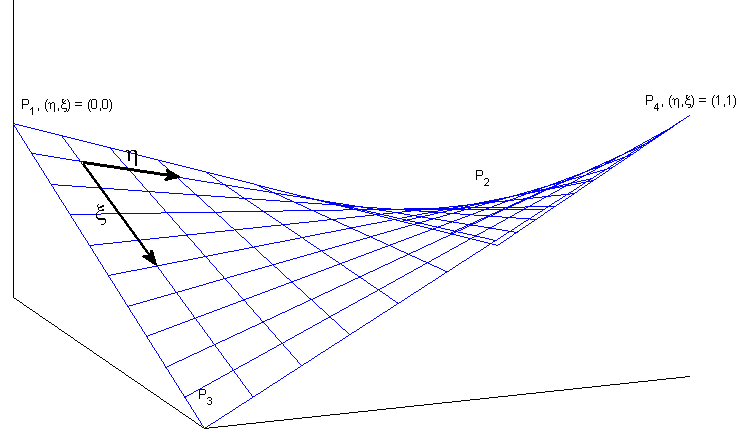
\includegraphics[width = 10cm]{gfx/bilinearSurface}
	\caption{Mathematically, a the chord face of a wing segment is a bilinear surface}
	\label{fig:bilin_surf}
\end{figure}

\subsection{Parametrization of the chord surface}

For simplicity, lets rename $\alpha := \eta$, $\beta := \xi$. Each point $\vec p$ on the surface then be expressed by

\begin{align}
\vec p(\alpha, \beta) &= \left( \vec {p_1} (1-\alpha) + \vec {p_2} \alpha \right) (1-\beta) \\
                  &+ \left( \vec {p_3} (1-\alpha) + \vec {p_4} \alpha \right) \beta \\
                  &= \alpha \underbrace{(-\vec p_1 + \vec p_2)}_{\vec a} + \beta\underbrace{(-\vec p_1 + \vec p_3)}_{\vec b} + \alpha \beta \underbrace{(\vec p_1 - \vec p_2 - \vec p_3 + \vec p_4)}_{\vec c} + \underbrace{\vec p_1}_{\vec d}
\label{eq:param}
\end{align}

This formula defines the transformation between the segments coordinates $(\alpha, \beta)$ to cartesian coordinates $(x, y, z)$. Mathematically, this form is called called bilinear surface. To sum up:

\begin{align}
\vec p (\alpha, \beta) &= \alpha   \vec a + \beta \vec b + \alpha \beta \vec c + \vec d \, , \quad
\textrm{with}\\
\vec a &= -\vec p_1 + \vec p_2 \nonumber \\
\vec b &= -\vec p_1 + \vec p_3 \nonumber \\
\vec c &= \vec p_1 - \vec p_2 - \vec p_3 + \vec p_4 \nonumber \\
\vec d &= \vec p_1 \nonumber
\end{align}

\subsection{Projecting a point onto the chord surface}
The projection of a point $\vec x$ onto the surface is defined as the point $\vec p(\alpha, \beta)$ so that $\vec p (\alpha, \beta) - \vec x$ is orthogonal to the surface. Mathematically it can be shown, that the orthogonality requirement is equivalent to finding the point $\vec p(\alpha, \beta)$ that has a smallest distance to $\vec x$. \par
This is of course an optimization problem which can be defined as:
\begin{equation}
\min_{\alpha, \beta} f(\alpha, \beta) := \min_{\alpha, \beta} \Vert \vec p(\alpha, \beta) - \vec x \Vert^2
\end{equation}
This is an almost quadratic problem (it is only quadratic, if $\vec c = 0$) and can be thus solved with Newton's optimization method. Newtons method is an iterative procedure. In our case, we can adapt it as follows:

\begin{algorithm}[htb]
 %\SetAlgoLined
 $(\alpha; \beta)_0 \leftarrow (0; 0)$ \\
 $k \leftarrow 0$\\
 \While{not converged}{
  $(\alpha, \beta)_{k+1} \leftarrow (\alpha, \beta)_{k} - s [\nabla^2 f(\alpha, \beta) ]^{-1} \cdot \vec \nabla f(\alpha, \beta),\quad \textrm{with}\, s \leq 1$\\
  $k \leftarrow k + 1$ \\
 }
 \caption{Newton's optimization algorithm}
\end{algorithm}

 
In order to perform this projection, we need the gradient $\vec \nabla f(\alpha, \beta)$ and the hessian matrix $\nabla^2 f(\alpha, \beta)$, which are defined as the first and second order derivative of $f(\alpha, \beta)$. \\

\paragraph{Gradient}
Using the chain rule, we get for the gradient:
\begin{equation}
\vec \nabla f(\alpha, \beta) = 2 J_p (\alpha, \beta)^T \cdot (\vec p(\alpha, \beta) - \vec x),
\end{equation}
where $J_p (\alpha, \beta)$ is the Jacobian of $\vec p(\alpha, \beta)$. In components this is:
\begin{align}
\frac {\partial f} {\partial \alpha}(\alpha, \beta) &= 2 \left(\frac{\partial \vec p}{\partial \alpha}(\alpha, \beta)\right)^T (\vec p(\alpha, \beta) - \vec x) \nonumber\\
&= 2\left( \vec a + \beta \vec c \right)^T (\vec p(\alpha, \beta) - \vec x) 
\end{align}
and
\begin{align}
\frac {\partial f} {\partial \beta}(\alpha, \beta) &= 2 \left(\frac{\partial \vec p}{\partial \beta}(\alpha, \beta)\right)^T (\vec p(\alpha, \beta) - \vec x) \nonumber\\
&= 2\left( \vec b + \alpha \vec c \right)^T (\vec p(\alpha, \beta) - \vec x) 
\end{align}

\paragraph{Hessian}
A derivative of the gradient gives as the Hessian matrix:
\begin{align}
\nabla^2 f(\alpha, \beta) = 2 J_p (\alpha, \beta)^T J_p (\alpha, \beta) + 2 (\nabla^2 \vec p (\alpha, \beta))^T \cdot (\vec p(\alpha, \beta) - \vec x)
\end{align}
Thus for the diagonal elements of the Hessian, we get
\begin{align}
\frac {\partial^2 f} {\partial \alpha^2}(\alpha, \beta) &= 2(\vec a + \beta \vec c)^T(\vec a + \beta \vec c) = 2 \Vert \vec a + \beta \vec c \Vert^2 \\
\frac {\partial^2 f} {\partial \beta^2}(\alpha, \beta) &= 2(\vec b + \alpha \vec c)^T(\vec b + \alpha \vec c) = 2 \Vert \vec b + \alpha \vec c \Vert^2 
\end{align}
and for the off-diagonals
\begin{align}
\frac {\partial^2 f} {\partial \alpha \partial  \beta}(\alpha, \beta) 
&= 2(\vec a + \beta \vec c)^T(\vec b + \alpha \vec c) + 2(\vec p (\alpha, \beta) - \vec x)^T \vec c.
\end{align}
Due to the symmetry of the Hessian, we get the same result for the other off-diagonal element $\frac {\partial^2 f} {\partial \beta \partial  \alpha}(\alpha, \beta)$.
\section{Component segment coordinate transform}
%
\begin{figure}[htb]
  \centering
  % trim left, bottom, right , top
  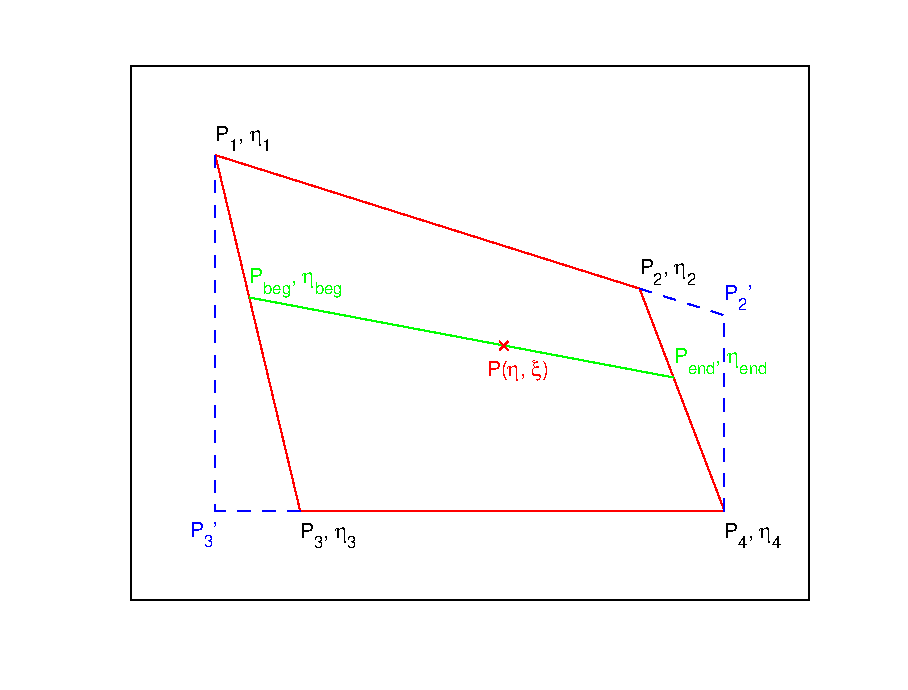
\includegraphics[trim=1cm 1cm 1cm 0.5cm, clip=true,width = 8cm]{gfx/compSegTheo}
	\caption{Illustration for the calculation of the component segment coordinate transformation}
	\label{fig:cs_surf}
\end{figure}
%
The coordinate transform of component segment coordinates is somewhat more complicated than the segment coordinate transform. To simplify the procedure, the component segment should consist of only one segment for now. The segment is again defined by its corner points $\vec p_1 \dots \vec p_4$. Figure \ref{fig:cs_surf} should help understanding the forthcoming calculations. \par
First we need some definitions:
\begin{itemize}
	\item Leading edge:  $ \vec s_v = \vec p_2 - \vec p_1 $
	\item Trailing edge: $ \vec s_h = \vec p_4 - \vec p_3 $
	\item Projected leading edge:   $\vec n = -\vec s_v$, with $n_x = 0$  
\end{itemize}


\subsection{Extending leading and trailing edges}
Plane through $\vec p_4$ with normal vector $\vec n$. Calculate inersection with leading edge. Plane equation is:
\begin{equation}
(\vec p - \vec p_4) \cdot \vec n = 0
\label{eq:plane}
\end{equation}
 Linear equation for the leading edge:
 
\begin{equation}
\vec p = \vec p_1 + \alpha (\vec p_2 - \vec p_1)
\label{eq:lin_eq1}
\end{equation}

Inserting (\ref{eq:lin_eq1}) into (\ref{eq:plane}) yields:
\begin{equation}
\alpha_v = \frac {(\vec p_4 - \vec p_1) \cdot \vec n }{(\vec p_2 - \vec p_1) \cdot \vec n}
\label{eq:nothing}
\end{equation}
%
If $\alpha_v > 1$, the leading edge has to be extended, else the trailing edge must be extended. In the first case, we calculate the extended leading edge point $\vec p_2^\prime$:
\begin{equation}
\vec p_2^\prime = \vec p_1 + \alpha_v (\vec p_2 - \vec p_1)
\label{eq:}
\end{equation}
%
In the other case ($\alpha_v < 1$), the intersection point with the trailing edge can be calculated in the same fashion.  \par
Now, we apply the same method also to the inner section, getting the extended points $\vec p_1^\prime$ and $\vec p_2^\prime$.

\subsection{Calculating $\eta$ values of the corners}
For the following calculations, we need to know the eta coordinates of the corner points $\vec p_1 \dots \vec p_4$. Lets image a plane with the previously defined normal vector $\vec n$ that goes through one of these points. Without loss of generality, let this point be $\vec p_3$. This plane is then defined by the equation
%
\begin{equation}
(\vec p - \vec p_3) \cdot \vec n = 0
\label{eq:plane_p3}
\end{equation}
%
Now we should find out, at which eta coordinate the plane intersects the leading edge, which is now parametrized as follows:
\begin{equation}
p = \vec p_1^ \prime + \eta ({\vec p_2}^\prime - {\vec p_1}^\prime).
\end{equation}
Combining both equations leads to $\eta_3 = \frac {(\vec p_3 - {\vec p_1}^\prime) \cdot \vec n }{({\vec p_2}^\prime - {\vec p_1}^\prime) \cdot \vec n}$, or in general:
\begin{equation}
\eta_i = \frac {(\vec p_i - {\vec p_1}^\prime) \cdot \vec n }{({\vec p_2}^\prime - {\vec p_1}^\prime)\cdot \vec n}.
\end{equation}

After doing these calculations (which have to be done only once), we can finally proceed to the coordinate transform.

\subsection{Calculating 3D coordinates of the $(\eta, \xi)$ pair}
The easiest way to do the transformation is to move first in $\xi$ direction. As the component segment is straight between the points $(\vec p_1, \vec p_3)$ and $(\vec p_2, \vec p_4)$ by definition, we move first along these lines:
\begin{align}
\vec p_{beg}(\xi) &= (1-\xi)\vec p_1 + \xi \vec p_3 \\
\vec p_{end}(\xi) &= (1-\xi)\vec p_2 + \xi \vec p_4
\end{align}

The corresponding eta coordinates of the points are 
\begin{align}
\eta_{beg}(\xi) &= (1-\xi)\eta_1 + \xi \eta_3 \\
\eta_{end}(\xi) &= (1-\xi)\eta_2 + \xi \eta_4
\end{align}

Finally, we walk along the line defined by the new point $\vec p_{beg}$ and $\vec p_{end}$ (depicted green in figure \ref{fig:cs_surf}). We have to keep in mind their eta coordinates (which are not 0 and 1)! We get our final result

\begin{equation}
\vec p(\eta, \xi) = \vec p_{beg} (\xi) + \frac {\eta - \eta_{beg}(\xi)}{\eta_{end}(\xi) - \eta_{beg}(\xi)} \cdot \left( \vec p_{end}(\xi) - \vec p_{beg}(\xi) \right).
\end{equation}

%\input{FileName} %You need a file 'FileName.tex' for this.


\end{document}

